\documentclass[border=10pt]{standalone}

\usepackage{tikz}
\usepackage{tikzsymbols}
\usetikzlibrary{calc,patterns,shapes.geometric}

\def\centerarc[#1](#2)(#3:#4:#5){\draw[#1] ($(#2)+({#5*cos(#3)},{#5*sin(#3)})$) arc (#3:#4:#5);}

\begin{document}
	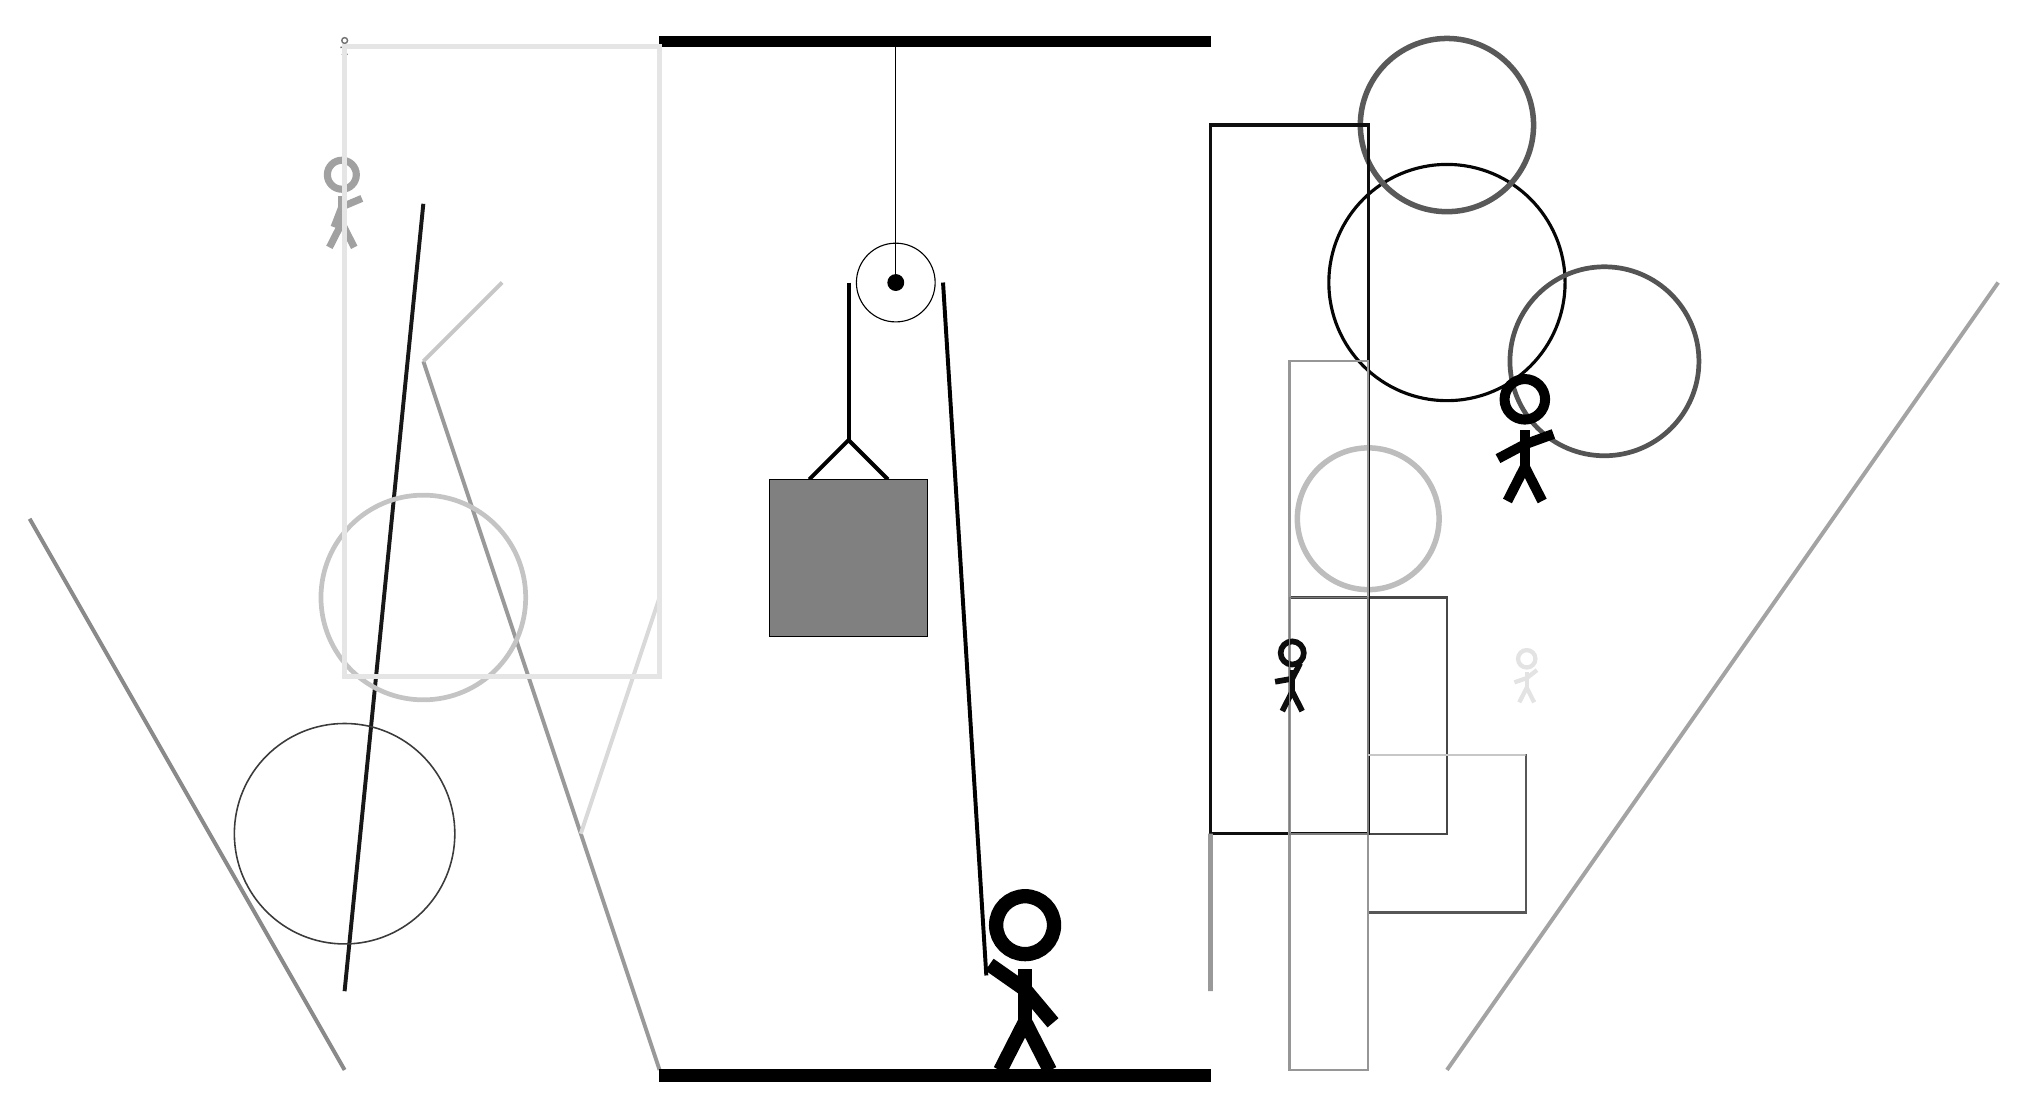
\begin{tikzpicture}
		%%%%% START %%%%%
		
		\draw[fill=black] (-2, 10) rectangle (5, 10.125);
		
		\draw (1, 7) circle (0.5);
		\draw[fill=black] (1, 7) circle (0.1);
		\draw (1, 10) -- (1, 7);
		
		\draw[line width=0.5mm] (-0.1, 4.5) -- (0.4, 5.0) -- (0.9, 4.5);
		\draw[fill=black!50] (-0.6, 4.5) rectangle (1.4, 2.5);
		
		\draw[line width=0.5mm] (0.4, 7) -- (0.4, 5.0);
		\centerarc[line width=0.5mm](1, 7)(0:180:0.6);
		\draw[line width=0.5mm](1.6, 7) -- (2.15, -1.8);
		
		\node[line width=0.3mm, color=black!55] at (-6, 10) {\Strichmaxerl[1][6][17]};
		
		\draw [line width=0.7mm, color=black!26](7, 4) circle (0.9);
		\draw[line width=0.3mm, color=black!66] (7, -1) rectangle (9, 1);
		\draw [line width=0.4mm, color=black!98](8, 7) circle (1.5);
		
		\draw[line width=0.5mm, color=black!46](-6, -3) -- (-10, 4);
		\draw[line width=0.5mm, color=black!40](-2, -3) -- (-5, 6);
		\node[line width=0.6mm, color=black!11] at (9, 2) {\Strichmaxerl[3][19][38]};
		\draw[line width=0.5mm, color=black!91](-6, -2) -- (-5, 8);
		\draw[line width=0.5mm, color=black!36](8, -3) -- (15, 7);
		\draw[line width=0.3mm, color=black!72] (6, 0) rectangle (8, 3);
		
		\draw [line width=0.2mm, color=black!77](-6, 0) circle (1.4);
		\draw[line width=0.5mm, color=black!22](-4, 7) -- (-5, 6);
		\draw [line width=0.7mm, color=black!65](8, 9) circle (1.1);
		
		\draw[line width=0.4mm, color=black!94] (7, 0) rectangle (5, 9);
		\draw [line width=0.6mm, color=black!67](10, 6) circle (1.2);
		\draw [line width=0.6mm, color=black!23](-5, 3) circle (1.3);
		
		\draw[line width=0.5mm, color=black!15](-2, 3) -- (-3, 0);
		\draw[line width=0.3mm, color=black!41] (6, -3) rectangle (7, 6);
		\node[line width=0.4mm, color=black!95] at (6, 2) {\Strichmaxerl[4][10][63]};
		\draw[line width=0.6mm, color=black!40] (5, 0) rectangle (5, -2);
		\draw[line width=0.2mm, color=black!51] (7, 0) rectangle (6, 3);
		
		\node[line width=0.7mm, color=black!37] at (-6, 8) {\Strichmaxerl[5][69][23]};
		
		\draw[line width=0.3mm, color=black!22] (7, 1) rectangle (9, 1);
		\draw[line width=0.6mm, color=black!10] (-2, 2) rectangle (-6, 10);
		\node[line width=0.4mm, color=black!100] at (9, 5) {\Strichmaxerl[7][28][20]};
		
		\node at (2.6, -1.9) {\Strichmaxerl[10][-35][-50]};
		
		\draw[fill=black] (-2, -3) rectangle (5, -3.15);
		
		%%%%% END %%%%%
	\end{tikzpicture}
\end{document}